%%=============================================================================
%% Inleiding
%%=============================================================================

\chapter{\IfLanguageName{dutch}{Inleiding}{Introduction}}%
\label{ch:inleiding}

%De inleiding moet de lezer net genoeg informatie verschaffen om het onderwerp te begrijpen en in te zien waarom de onderzoeksvraag de moeite waard is om te onderzoeken. In de inleiding ga je literatuurverwijzingen beperken, zodat de tekst vlot leesbaar blijft. Je kan de inleiding verder onderverdelen in secties als dit de tekst verduidelijkt. Zaken die aan bod kunnen komen in de inleiding~\autocite{Pollefliet2011}:
%
%\begin{itemize}
%  \item context, achtergrond
%  \item afbakenen van het onderwerp
%  \item verantwoording van het onderwerp, 

%  \item probleemstelling
%  \item onderzoeksdoelstelling
%  \item onderzoeksvraag
%  \item \ldots
%\end{itemize}

\section{\IfLanguageName{dutch}{Probleemstelling}{Problem Statement}}%
\label{sec:probleemstelling}

%Uit je probleemstelling moet duidelijk zijn dat je onderzoek een meerwaarde heeft voor een concrete doelgroep. De doelgroep moet goed gedefinieerd en afgelijnd zijn. Doelgroepen als ``bedrijven,'' ``KMO's'', systeembeheerders, enz.~zijn nog te vaag. Als je een lijstje kan maken van de personen/organisaties die een meerwaarde zullen vinden in deze bachelorproef (dit is eigenlijk je steekproefkader), dan is dat een indicatie dat de doelgroep goed gedefinieerd is. Dit kan een enkel bedrijf zijn of zelfs één persoon (je co-promotor/opdrachtgever).

Bij het opnemen van een vak worden studenten aan de HOGENT tijdens het semester vaak geconfronteerd met een grote hoeveelheid aan informatie: lesmodaliteiten, opdrachten, deadlines en kennismaking met de benodigde software, om slechts enkele voorbeelden te noemen. Dit leidt ertoe dat er gedurende het semester regelmatig vragen ontstaan. Om antwoorden te vinden, onderscheiden veel studenten twee belangrijke informatiebronnen: enerzijds de officiële bronnen die door de hogeschool worden aangeboden, en anderzijds de informatie die studenten onderling met elkaar uitwisselen.

Vanuit de hogeschool worden verschillende informatiebronnen aangeboden waarop studenten en docenten antwoorden kunnen vinden op hun vragen. Ten eerste is er de studiewijzer van het vak. Hierin is informatie te vinden over eventueel aan te schaffen materialen, mogelijke softwarevereisten, deadlines en de organisatie van het vak. Daarnaast zijn er de aangeboden studiematerialen, zoals slides, syllabi, handboeken en dergelijke, die de vakinhoud behandelen. Verder zijn er de studiefiches, waarin algemene informatie staat zoals de studielast, de leerresultaten en de evaluatievorm. Bij sommige vakken worden ook aanvullende bestanden verstrekt die studenten begeleiden bij bepaalde onderwerpen en vaak voorkomende problemen of vragen behandelen. Tot slot is bij sommige vakken ook een forum beschikbaar. Dit forum dient als centrale plaats om vragen te stellen, waarbij de antwoorden zichtbaar zijn voor alle studenten.

Daarnaast maken veel mensen gebruik van sociale media om informatie over specifieke onderwerpen uit te wisselen, en studenten vormen hierop geen uitzondering. Sociale media wordt ingezet om met andere studenten over de vakinhoud te communiceren en zo nieuwe kennis op te doen. Deze veronderstelling is ook bevestigd in andere onderzoeken. \textcite{M.Talaue2018} en \textcite{Bal2017} interviewden verschillende studenten over hun gebruik van sociale media, waaruit blijkt dat een groot deel van hen sociale media gebruikt om vakken hun inhoud te bespreken. Aan de HOGENT is dit eveneens het geval. Naast hun persoonlijke profielen op andere media, komen studenten samen op een \emph{Discord}-server. Deze server is onderverdeeld in verschillende kanalen, waarbij elk kanaal een specifiek vak vertegenwoordigt. Studenten bespreken in deze kanalen alles wat met het desbetreffende vak te maken heeft en stellen er hun vragen. Aangezien deze server door studenten wordt beheerd en docenten er geen toegang toe hebben, omdat het \emph{geen officieel kanaal van HOGENT} is, bestaat het risico dat er foutieve informatie wordt uitgewisseld. Een voorbeeld van een dergelijk scenario is te zien in Figuur~\ref{fig:misinformatie_discord}. Hier vindt een uitwisseling plaats tussen twee studenten over het vak \emph{The IT Professional \& Career Orientation}. De tweede student deelt foutieve informatie met de eerste, zoals blijkt uit de aankondiging op Chamilo, die wél de juiste informatie bevat.

\begin{figure}
    \centering
    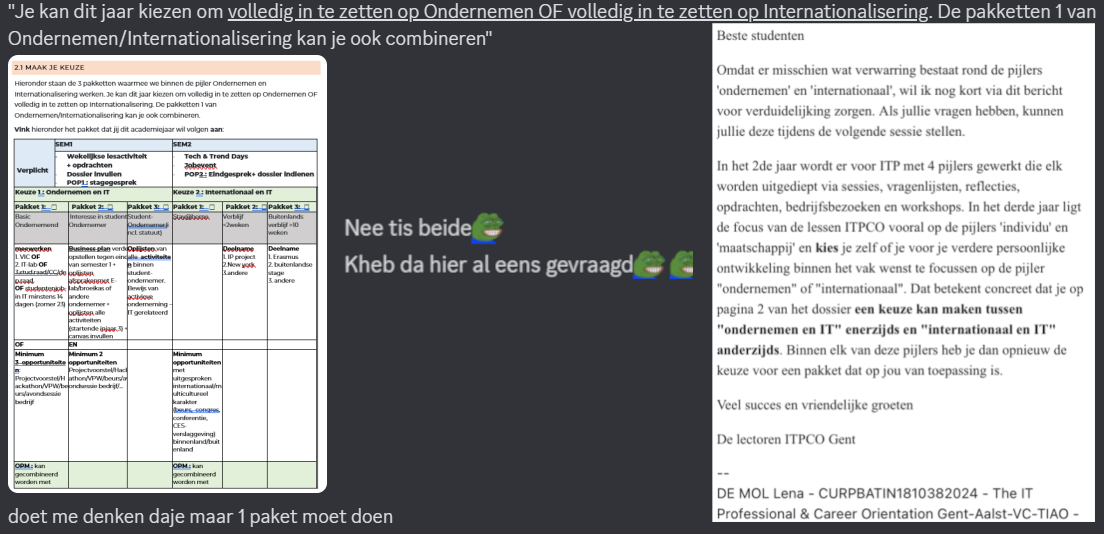
\includegraphics[width=0.9\textwidth]{misinformatie_discord.png}
    \caption[Misinformatie op Discord-server]{\label{fig:misinformatie_discord}Vraag dat gesteld werd op de Discord-server en die een foutieve antwoord kreeg van een medestudent. De correcte informatie werd gecommuniceerd in een aankondiging op Chamilo.}
\end{figure}

Zoals blijkt, is informatie verspreid over een verscheidenheid aan media. Informatie vinden kan daarom enige moeite kosten, en de kans op onduidelijkheden of tegenstrijdige informatie is aanzienlijk. In het geval van problemen is het laatste redmiddel voor studenten om contact op te nemen met de docent. De positie van docenten stelt hen in staat om onduidelijkheden te verhelderen, maar zij hebben hier niet altijd de tijd voor, waardoor studenten mogelijk hun antwoord niet op tijd ontvangen. Bovendien kan het herhaaldelijk beantwoorden van dezelfde vragen frustrerend zijn.

Er bestaat dus behoefte aan een middel dat de belasting voor alle betrokken partijen verlicht door antwoorden te bieden op de veelgestelde vragen van studenten en deze antwoorden on-demand levert. 

\section{\IfLanguageName{dutch}{Onderzoeksvraag}{Research question}}%
\label{sec:onderzoeksvraag}

%Wees zo concreet mogelijk bij het formuleren van je onderzoeksvraag. Een onderzoeksvraag is trouwens iets waar nog niemand op dit moment een antwoord heeft (voor zover je kan nagaan). Het opzoeken van bestaande informatie (bv. ``welke tools bestaan er voor deze toepassing?'') is dus geen onderzoeksvraag. Je kan de onderzoeksvraag verder specifiëren in deelvragen. Bv.~als je onderzoek gaat over performantiemetingen, dan 

Dankzij de technologische vooruitgang van de afgelopen jaren staat het vakgebied van \acrfull{AI} opnieuw in de schijnwerpers. \acrlong{AI} wordt toegepast in een verscheidenheid aan domeinen, vaak met indrukwekkende resultaten. Onder al deze toepassingen lijkt het taaldomein echter de meest opmerkelijke vooruitgang te boeken, wat heeft geleid tot de geboorte van \acrfull{LLM} (zie~\ref{sec:llms}).
 
\acrshort{LLM}'s zijn modellen die in staat zijn om menselijke taal te begrijpen en te genereren. Het bekendste voorbeeld is ongetwijfeld de \emph{\gls{GPT-modellen}}. Deze modellen, waarop de chatbot \emph{ChatGPT} gebaseerd is, veroverden de wereld in sneltempo dankzij hun vermogen om mensachtige gesprekken te voeren en de brede waaier aan taken die ze kunnen uitvoeren. Deze revolutie heeft geleid tot het ontstaan van een nieuwe generatie chatbots die gebruikmaken van \acrshort{LLM}'s als onderliggende technologie (zie~\ref{sec:chatbots}). In onze zoektocht naar een oplossing voor het hierboven beschreven probleem, lijken dergelijke chatbots een veelbelovende uitkomst te bieden.

In deze bachelorproef wordt de haalbaarheid onderzocht van Eureka, een virtuele assistent die studenten en docenten ondersteunt bij het beantwoorden van vakgerelateerde vragen, evenals de toepasbaarheid ervan binnen de context van de vakken\emph{Data Science \& AI}, \emph{Infrastructure automation} en \emph{Linux for Data Scientists}. Met andere woorden, we trachten na te gaan of een dergelijke chatbot een geschikte oplossing biedt voor het voorliggende probleem en in welke mate deze effectief is.
 
\section{\IfLanguageName{dutch}{Onderzoeksdoelstelling}{Research objective}}%
\label{sec:onderzoeksdoelstelling}

%Wat is het beoogde resultaat van je bachelorproef? Wat zijn de criteria voor succes? Beschrijf die zo concreet mogelijk. Gaat het bv.\ om een proof-of-concept, een prototype, een verslag met aanbevelingen, een vergelijkende studie, enz.

De haalbaarheid en toepasbaarheid van Eureka worden getoetst aan de hand van een \emph{Proof-of-Concept} (PoC). Deze PoC moet aan bepaalde criteria voldoen, zowel vanuit het probleemdomein als het oplossingsdomein, om als succesvol te worden beschouwd. Deze criteria vloeien voort uit de verwachtingen die studenten en docenten hebben van een dergelijke tool.

Betreffende het probleemdomein wordt verwacht dat Eureka relevante antwoorden genereert; dit is immers de bestaansreden van deze tool. De bron van het antwoord moet ook worden meegedeeld, zodat de student of docent de betrouwbaarheid van de informatie kan verifiëren en deze verder kan doorzoeken indien gewenst. Daarnaast wordt verwacht dat hallucinaties (zie~\ref{subsec:valkuilen}) strikt worden vermeden. Als valse informatie wordt verspreid, leidt dit tot meer verwarring en werkt het tegen het nut van deze tool in.

Ten slotte wordt ook verwacht dat Eureka onverwachte interacties, zoals beledigingen, aankan. De menselijke natuur is onvoorspelbaar en dergelijke interacties zullen zich voordoen. Eureka moet hier robuust tegen zijn.

Voor het oplossingsdomein wordt verwacht dat Eureka op een eenvoudige manier kan worden uitgebreid of gewijzigd. De schoolomgeving is zeer dynamisch en wijzigingen komen regelmatig voor. Deze wijzigingen moeten snel kunnen worden doorgevoerd in Eureka en op een gebruiksvriendelijke manier, zodat ook docenten zonder gespecialiseerde technische kennis of expertise in het vakgebied dit kunnen doen.

Bovendien moet de toepassing van Eureka rekening houden met de beperkte financiële en computationele middelen waarover we beschikken.

\section{\IfLanguageName{dutch}{Opzet van deze bachelorproef}{Structure of this bachelor thesis}}%
\label{sec:opzet-bachelorproef}

% Het is gebruikelijk aan het einde van de inleiding een overzicht te
% geven van de opbouw van de rest van de tekst. Deze sectie bevat al een aanzet
% die je kan aanvullen/aanpassen in functie van je eigen tekst.

De rest van deze bachelorproef is als volgt opgebouwd:

In Hoofdstuk~\ref{ch:literatuurstudie} onderzoeken we de stand van zaken binnen het onderzoeksdomein op basis van een literatuurstudie. Hierin geven we een kort overzicht van de geschiedenis van chatbots en zien we dat de huidige generatie chatbots gebaseerd is op \acrshort{LLM}'s. Daarna bespreken we wat \acrshort{LLM}'s zijn. Aangezien we een chatbot willen ontwerpen voor een specifieke use-case binnen HOGENT, bestuderen we hoe een \acrshort{LLM} gespecialiseerd kan worden en wat er allemaal komt kijken bij de gekozen techniek. Uiteindelijk sluiten we de literatuurstudie af door de mogelijke valkuilen te benoemen die kunnen optreden bij het implementeren van dergelijke technologie.

In Hoofdstuk~\ref{ch:methodologie} wordt de methodologie toegelicht. Hier bespreken we hoe het onderzoek is opgedeeld. Het onderzoek bestaat uit een ontdekkingsfase, een implementatiefase en een testfase.

De ontdekkingsfase heeft als doel een \acrshort{LLM} te vinden die aan bepaalde verwachtingen voldoet. Deze fase wordt uitgevoerd in een beperkte en gecontroleerde omgeving.

De implementatiefase omvat de daadwerkelijke implementatie van Eureka. Hierbij wordt een pijplijn opgebouwd, samengesteld uit verschillende componenten. Elk van deze componenten en hun functie worden verder toegelicht.

Tijdens de testfase wordt Eureka geëvalueerd aan de hand van de gestelde verwachtingen. Hiervoor worden persona's gebruikt.

Bij elke fase wordt ook een ingeschatte duurtijd vermeld.

% TODO: Vul hier aan voor je eigen hoofstukken, één of twee zinnen per hoofdstuk

In Hoofdstuk~\ref{ch:conclusie}, tenslotte, wordt de conclusie gegeven en een antwoord geformuleerd op de onderzoeksvragen. Daarbij wordt ook een aanzet gegeven voor toekomstig onderzoek binnen dit domein.